\documentclass[laboratorio]{guia}

\def \practnum {4} 
\def \practica {Ley de Inducci\'on de Faraday}

\def \materia {Laboratorio de F\'\i sica II para Qu\'\i micos}
\def \periodo {2\sptext{o} cuatrimestre de 2016}
\def \profesor {Diana Skigin}
\def \website {http://materias.df.uba.ar/f2qa2016c2}
 
\usepackage{graphics}
\usepackage{amsmath}
\usepackage{amsfonts}
\usepackage{graphicx}
\usepackage{float}
\usepackage{wrapfig}
\usepackage{subfigure}
\usepackage{bm}
\usepackage{grffile}
\usepackage{color}
\usepackage{framed}
\usepackage[utf8]{inputenc}
\usepackage[T1]{fontenc}
\usepackage{lmodern} 
% definicion del entorno 'sabermas'
\makeatletter
\definecolor{shadecolor}{rgb}{0.89,0.91,0.94}
\newenvironment{sabermas}[1]{%
\vfill
\begin{shaded}
  \begin{center}
  {\textsection{Para saber m\'as}}
  \end{center}
  #1
\sf } 
{%
\end{shaded}%
}
\makeatother

\renewcommand{\vec}[1]{\ensuremath{\mathbf{#1}}}




\hyphenation{ coe-fi-cien-tes coe-fi-cien-te au-to-va-lor
              au-to-va-lo-res co-rres-pon-der pro-ble-ma 
              cual-quie-ra po-la-ri-za-cio-nes }

\graphicspath{{./Guia_04_Induccion/}}

\begin{document} 
\objetivo{%
    El objetivo de esta gu\'\i a experimental consiste en medir la fuerza
    electromotriz inducida sobre un circuito empleando para ello un generador
    de funciones y un osciloscopio (o un sistema de adquisici\'on de se\~nales
    asistido por computadora).
    \tematicas{fuerza electromotriz, inducci\'on, ley de Faraday.}} 
\maketitle

\section{Primera parte: Inducci\'on entre una bobina y un im\'an permanente}

En esta primera parte se propone abordar y responder experimentalmente a la siguiente pregunta:
?`qu\'e sucede cuando el campo magn\'etico generado por un im\'an permanente
var\'\i a dentro de una bobina, por ejemplo cuando uno acerca o mueve un
im\'an? 

Para responder a este interrogante, conecte una bobina al osciloscopio y
registre (en funci\'on del tiempo) el voltaje que se induce en la misma cuando
se acerca un im\'an a su interior. Estudie tambi\'en c\'omo var\'\i a la fuerza
electromotriz inducida de acuerdo a c\'omo se mueve el im\'an (r\'apida o
lentamente). 

En esta parte de la gu\'\i a, a fin de poder observar una se\~nal temporal
corta (debida, por ejemplo, al movimiento repentino del im\'an), resulta
conveniente usar la funci\'on de disparo \'unico del osciloscopio. Consulte a
su docente acerca de c\'omo habilitar dicho modo de trabajo en el osciloscopio.

\section{Segunda parte: Inducci\'on entre dos bobinas}

El dispositivo experimental propuesto para esta parte se ilustra
esquem\'aticamente en la Figura~\ref{fig:1}. El mismo consiste de una bobina
con un n\'umero $N$ de espiras; este elemento constituye el denominado {\it
primario} del circuito. Dicha bobina se conecta a un generador de funciones a
trav\'es de una resistencia $R$ (de entre 50 y 500 $\Omega$). El prop\'osito de
incluir esta resistencia es el de limitar la corriente que circula por la
bobina; y a la vez poder medir la corriente $I$ que circula por el circuito
primario. 

\begin{figure}[t!]
    \centering
    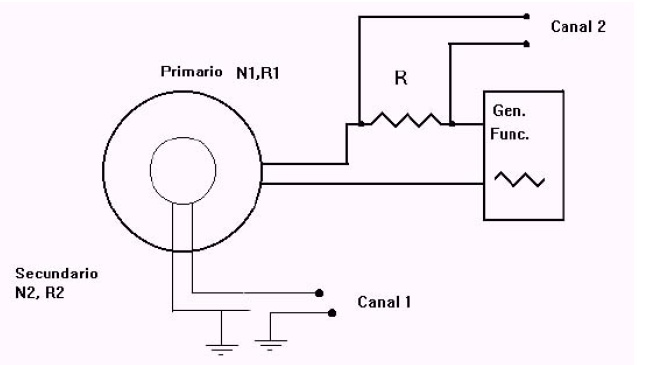
\includegraphics[width=8.5cm]{LG04--000.png}
    \caption{Esquema del dispositivo experimental propuesto para la segunda
    parte de la experiencia.}
    \label{fig:1}
\end{figure}

En general se debe evitar conectar cualquier fuente de tensi\'on (en este caso,
el generador de funciones) a elementos de poca impedancia (inferior a 50
$\Omega$), ya que se puede arruinar la fuente o quemar el circuito que \'esta
alimenta. 

A fin de realizar las mediciones, se propone el siguiente protocolo. En un
canal del osciloscopio se registra la ca\'\i da de tensi\'on $V_R$ en la
resistencia, a partir de lo cu\'al logramos obtener una se\~nal que resulta
proporcional a la corriente circulante. Se debe tener en cuenta al dise\~nar el
circuito que las tierras del generador de funciones y del osciloscopio deben
coincidir (?`por qu\'e?) Una segunda bobina con un n\'umero de espiras $M$ se conecta al otro canal del
osciloscopio; esta segunda bobina se denomina {\it el secundario} del presente
dispositivo.

A continuaci\'on coloque una bobina dentro de la otra de modo tal que el campo
magn\'etico generado en el primario entre dentro del bobinado del secundario.
Aplique entonces una tensi\'on sinusoidal al circuito de la Figura~\ref{fig:1}.
Estudie c\'omo var\'\i a la amplitud de tensi\'on inducida en el secundario
como funci\'on de la frecuencia del generador de funciones y luego en funci\'on
de la amplitud de tensi\'on del mismo.

Finalmente, se propone repetir la experiencia colocando ahora el n\'ucleo de
hierro en el interior de las bobinas. Describa en forma cualitativa la
relaci\'on entre las se\~nales de corriente del primario y tensi\'on del
secundario. Lleve a cabo esta experiencia con ondas sinusoidales y
triangulares. ?`Se puede decir que una se\~nal es la derivada de la otra?

\section{Tercera parte: Transformador}

Usando bobinas secundarias de diferente n\'umero de espiras, $N_2$, en los n\'ucleos de
hierro, pero manteniendo las condiciones del primario constantes (en amplitud y
frecuencia), investigue la dependencia de $V_2$ en funci\'on de $N_2$. ?`Qu\'e
concluye? 

El dispositivo formado por dos bobinas o espiras que comparten sus flujos se
conoce como {\it transformador}. Mida y represente el cociente de amplitudes
$V_2/V_1$ en funci\'on del cociente del n\'umero de espiras $N_2/N_1$. Indique
en forma esquem\'atica c\'omo har\'\i a para fabricar un transformador que
duplique la tensi\'on de l\'\i nea y otro que la reduzca en un factor 3. 

\nocite{Alonso1998,Purcell1988,Reitz1996,Trelles1984,Reitz1996}
\bibliographystyle{unsrt} 
\bibliography{Bibliografia}

\end{document}
